
	\centering
	\begin{tabular}{ |	p{30 mm}|	p{61 mm}	|	p{33mm}	| p{43mm}	| } 
		\hline
		
		
		\multirow{4}{30mm}{\centering 
\includegraphics[scale=0.22]{logo}} &
		\multirow{4}{61mm}{\centering \textbf{ \textbf{Manual de prácticas del Laboratorio de Análisis de Sistemas y Señales}}}    & Código: & MADO-76 \\
		\cline{3-4}
		& &  Versión & 01 \\
		\cline{3-4}
		& & Página: & 77/97 \\ \cline{3-4}
		& & Sección ISO: & 8.3 \\ \cline{3-4}
		& & Fecha de emisión: & 28 de frebrero 2019 \\
		\hline
	\end{tabular}
\begin{tabular}{ |	c |	c	| } 
	
	\multirow{2}{65mm}{ \centering Facultad de ingeniería} &
	\multirow{2}{111mm}{\centering \textbf{ Area/Departamento: \\ Laboratorio de control y robótica}}   \\
	& \\ \hline
\end{tabular}
\begin{tabular}{|p{180mm}|}
	\multirow{1}{180mm}{ \centering La impresion de este documento es una copia no controlada }  \\ \hline \end{tabular} \\

\vspace{1cm}


{\centering \LARGE Práctica N◦5 Respuesta de Sistemas Dinámicos }

\vspace{1.5cm}

\begin{figure}[!h]
	\centering
	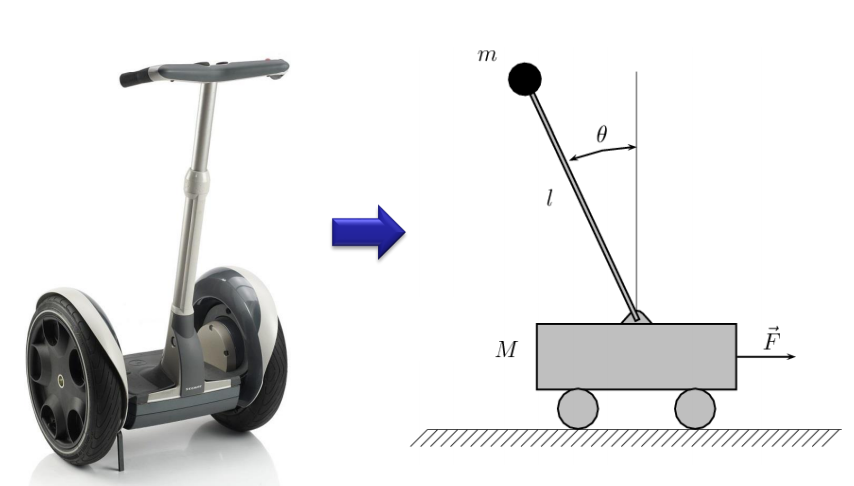
\includegraphics[scale=0.6]{portada.png}
\end{figure}

\hspace{2cm}

\hspace{1cm}
\begin{tabular}{|c| p{122mm}|}
	\hline
	\multirow{4}{50mm}{\\ \centering \large Apellidos y nombres}	 &  \\  
	& Alfaro Domínguez Rodrigo  \\  \cline{2-2}
	&  \\  
	& Barrera Peña Víctor Miguel \\  \cline{2-2}
	&  \\  
	& Villeda Hernández Erick Ricardo \\ 
	\hline
\end{tabular}
\begin{tabular}{|p{50mm} | c | p{80mm}| p{23mm} |}
	Grpo: & 4 & \multirow{2}{90mm}{Profesor: M.I Lauro Fernando Vazquez Alberto } & Calificación \\ \cline{1-2}
	Brigada: & 1 &  &\\ \hline
	Semestre: & 2021-1 & Fecha de ejecución: 05/01/2021 & \\ \hline
\end{tabular}




